\documentclass[a4paper]{article}
\usepackage{graphicx}
\usepackage{parskip}
\usepackage{titlesec}

\graphicspath{ {./img/} }
\titleformat{\section}[block]{\bfseries\filcenter}{}{1em}{}

\begin{document}
\title{Computer Architecture Lab 1 Report}
\author{Fabian Wüthrich}
\date{October 2020}
\maketitle

This lab examines the performance impact of different cache parameters. The
sample programs for the MIPS simulator are not well suited for cache exploration
as they are not memory intensive. Therefore, we added four memory-bound
benchmarks which are in the folder \verb|inputs/benchmark|. Here is a quick summary of
each benchmark:
\begin{description}
    \item[\texttt{stream}] A 64KB array is written sequentially and read back afterwards
    \item[\texttt{strided}] Strided access to a 64KB array
    \item[\texttt{locality}] Calculates the sum of an array. The sum is stored
        in memory and is accessed in every loop iteration (temporal locality)
    \item[\texttt{random}] Random access to a 64KB array
\end{description}
The following paragraphs describe different experiments to explore various cache
parameters. We consider only the data cache and use the parameters from the lab
sheet for the instruction cache.

\section{Cache Size}

For the first experiment, we fixed the block size to 4 bytes (one integer per
block) and used no associativity. The replacement policy is LRU. Then, we
measured the IPC for different cache sizes. The cache is disabled for a size of
zero, so every request has a memory latency. Figure \ref{fig:cache-size} shows
the result of this experiment. The IPC is normalized to the baseline with the
cache disabled.
\begin{figure}
    \centering
    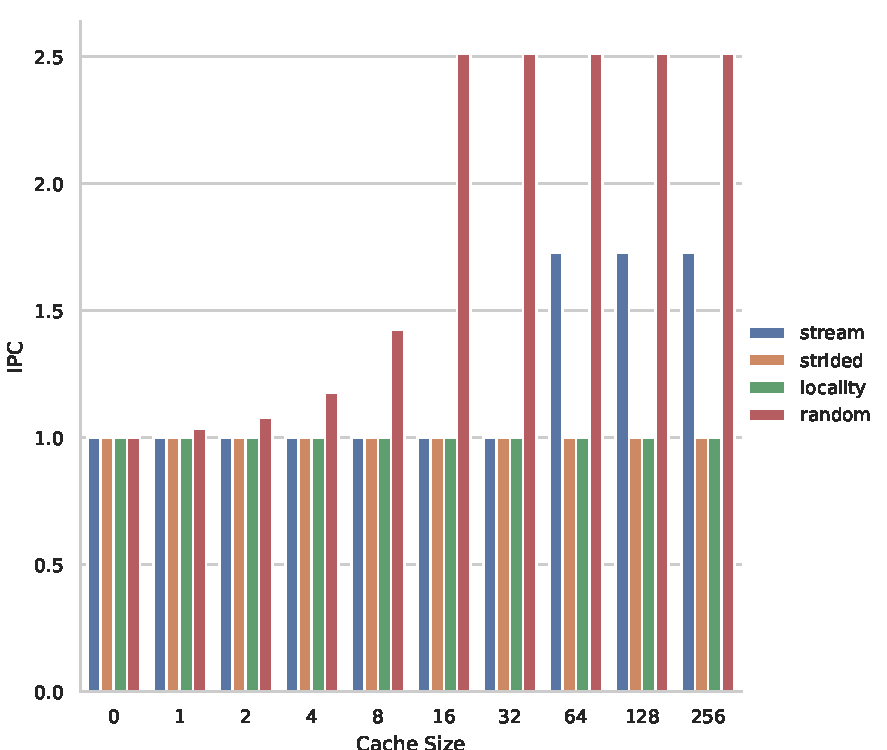
\includegraphics[width=\textwidth]{cache_size}
    \caption{Cache Size}
    \label{fig:cache-size}
\end{figure}

The plot shows that \texttt{stream} and \texttt{strided} are \textbf{equal to
system without a cache} for cache sizes below 64KB. The array does not fit in
cache for small sizes and chunks of the array override each other which explains
the poor performance. As soon as the \textbf{whole working set fits into cache}
(at 64KB), the \textbf{IPC increases} by 1.73 and does not improve further for
larger cache sizes.

The \texttt{locality} benchmark exceeds the baseline by 2.6x for all cache sizes.
The sum variable is rarely evicted from cache and the array has only compulsory
misses. Thus, \textbf{the cache size does not influence the performance} of this
benchmark.

For the random access, we get \textbf{a gradual performance increase} which stabilizes as
soon as the whole working set fits into cache. During random access, only parts
of the array are accessed. The probability of a hit increases with a larger cache
which explains the progressive increase.

\section{Block Size}

The second experiment examines the block size of the cache. We disabled
associativity and set the cache size to 64KB so that the whole array fits into
cache. The baseline has a block size of four. The results are shown in Figure
\ref{fig:block-size}.
\begin{figure}
    \centering
    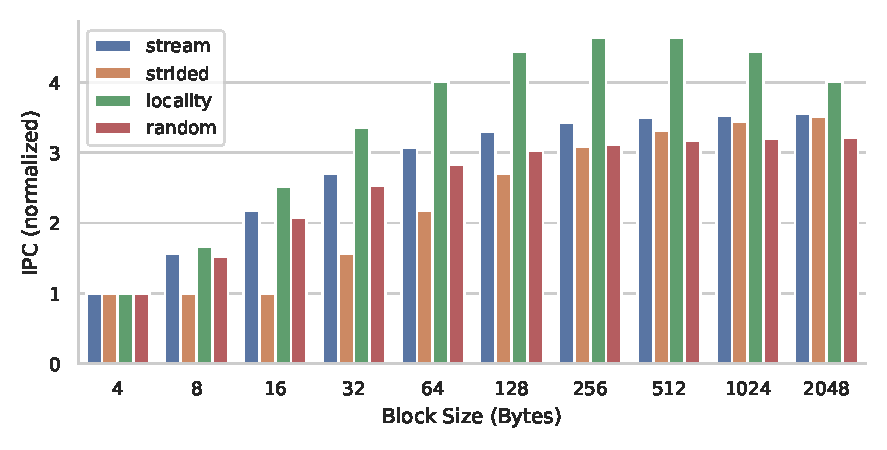
\includegraphics[width=\textwidth]{block_size}
    \caption{Block Size}
    \label{fig:block-size}
\end{figure}

We can see that the performance of \texttt{stream} and \texttt{random} \textbf{does
improve with higher block sizes}. Large blocks decrease compulsory misses and the
two benchmarks do not generate any conflicts, so the overall performance does
never decrease.

In contrast, the performance of \texttt{locality} \textbf{has a peak at 256/512KB and
decreases for larger block sizes}. With an increasing block size, more integers
are loaded into cache and at some point, the sum variable is evicted from cache
which explains the performance drop.

Finally, \texttt{strided} has up to 16 bytes a similar performance as the
baseline (one integer per block). If a block holds as many integers as the
stride, the performance starts to increase.

\section{Associativity}

The third experiment changes the associativity of the cache. Initially, we used
a cache size of 64KB and blocks of 4 bytes. With this configuration, all
benchmarks had the same IPC as the baseline (no associativity). We reduced the
cache size to 4KB to generate more conflicts. Figure \ref{fig:ways} shows that
only the \texttt{locality} benchmark \textbf{takes advantages of the cache
associativity}. All other benchmarks generate too few conflicts to benefit from
multiple ways.
\begin{figure}
    \centering
    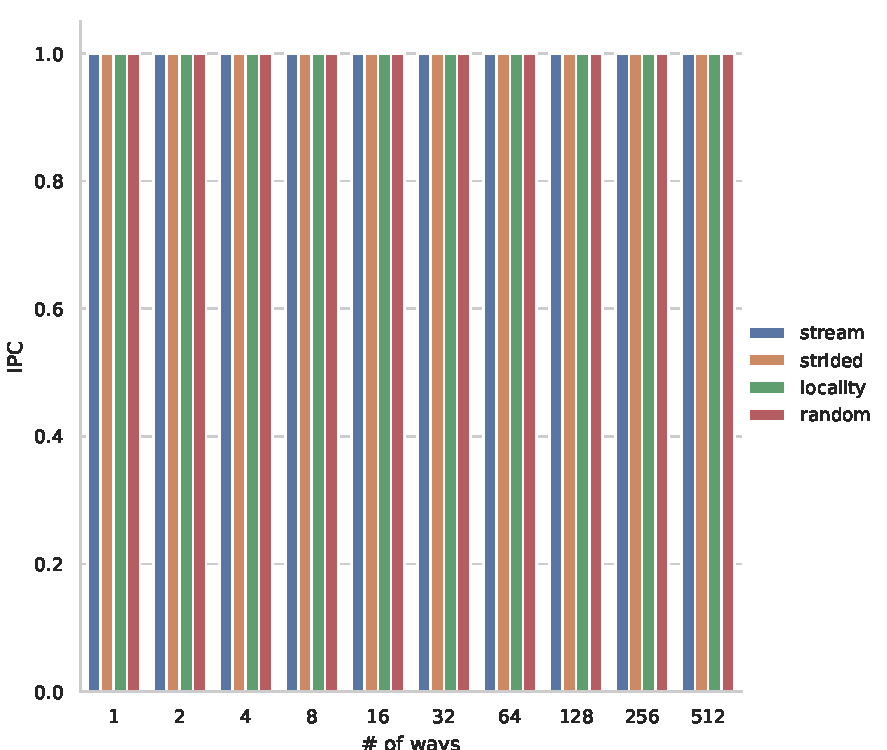
\includegraphics[width=\textwidth]{ways}
    \caption{Associativity}
    \label{fig:ways}
\end{figure}


\section{Replacement/Insertion Policies}

The last experiment tests different replacement and insertion policies. We
implemented different combinations of LRU and MRU policies. The combination is
labeled as \texttt{<replacement>\_<insertion>} in Figure \ref{fig:replacement}.
For example, \texttt{lru\_mru} means the least-recently used block is evicted
from cache and the new block is inserted as most-recently used. Additionally, we
added a FIFO and a LIFO policy.

The results in Figure \ref{fig:replacement} show that \textbf{the cache policy does not
influence the performance of any benchmark}. We experimented with various
cache/block sizes and associativities but the IPC (not normalized) of all
benchmarks remained the same for all policies. Eventually, we tried different
workloads and could observe performance improvements. We conclude that the
effectiveness of a cache policy is highly workload dependent.
\begin{figure}
    \centering
    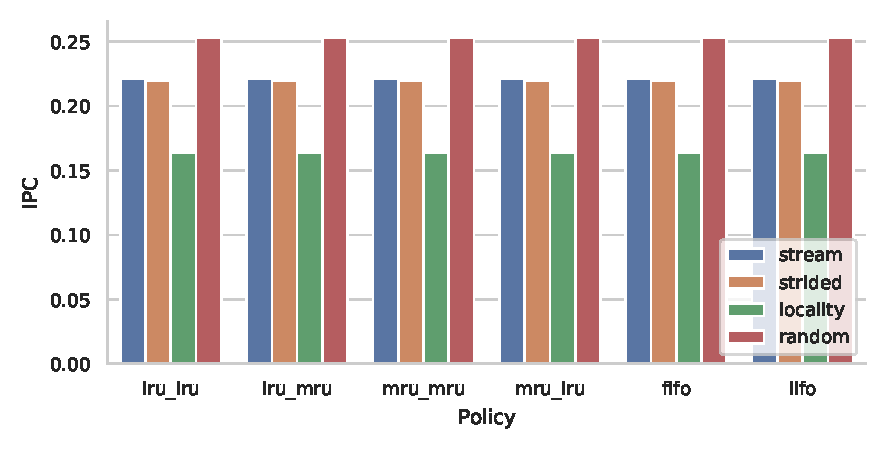
\includegraphics[width=\textwidth]{replacement}
    \caption{Cache Policies}
    \label{fig:replacement}
\end{figure}

\section{Most Performant Design}

Based on the previous experiments we derive an optimal cache configuration in
terms of performance. Firstly, we set the cache size to 64KB so that the whole
working set fits in cache. A larger cache does not improve performance for any
of the workloads. Secondly, we use a block size of 512 bytes. The performance of
\texttt{locality} drops for larger blocks whereas the other benchmarks have
a higher performance with an increasing block size. Finally, we use 2 ways to
support the \texttt{locality} benchmark and a LRU/MRU policy to stay in line
with the lab sheet.

The data cache in the lab sheet has an average IPC of 0.53, whereas our most
performant design has an average IPC of 0.78. Therefore, our optimized cache
configuration \textbf{outperforms the other cache by 47.1 \%.}

\end{document}
